\documentclass[10pt] {article}
\usepackage{fullpage}
\usepackage{amssymb}
\usepackage{graphicx}
\usepackage{float}
\usepackage{amsthm}
\usepackage{hyperref}
\usepackage{amsmath}
\renewcommand\qedsymbol{$\blacksquare$}

\title{Homework 3 }
\author{Ricky Hempel}
\begin{document}
\maketitle
\begin{center}
1.4a-c, 1.5b-d, 1.8b, 1.9a, 1.11, 1.14, 1.16, 1.18, 1.21, 1.28
\end{center}
\begin{enumerate}
\item[1.4]
a.Let the state diagram $M_1$ recognize 
$L_1 = \{ w \mid$ w has at least three a's $\}$:
\begin{figure}[H]
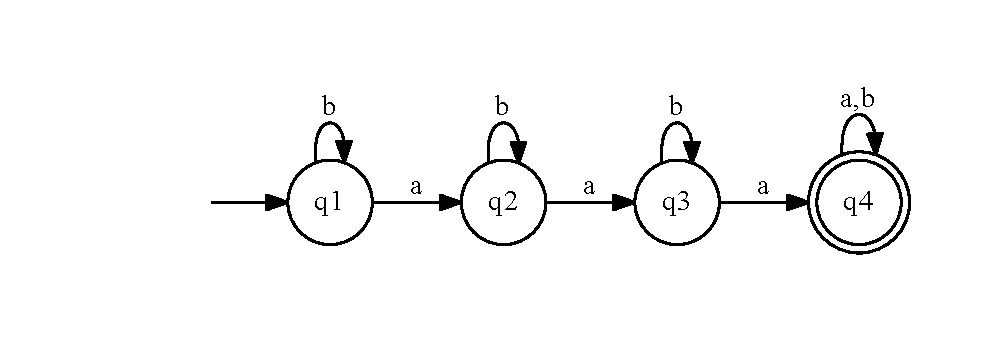
\includegraphics[width=0.9\textwidth]{a14.pdf}
\caption{State diagram for w has at least three a's.}
\label{1}
\end{figure} 
Let the state diagram $M_2$ recognize 
$L_2 = \{ w \mid$ w has at least twos b's $\}$:
\begin{figure}[H]
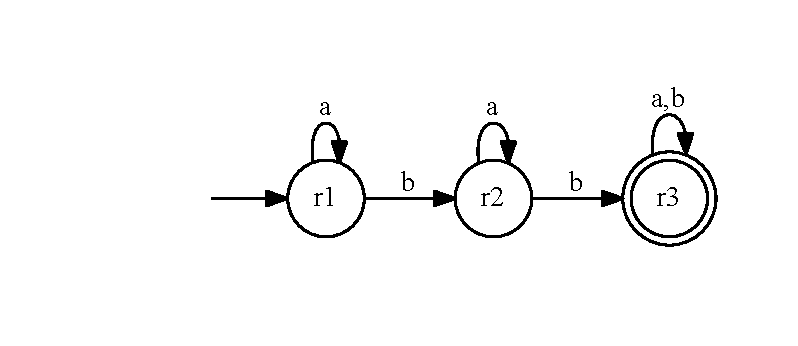
\includegraphics[width=0.9\textwidth]{ab14.pdf}
\caption{State diagram for w has at least two b's.}
\label{2}
\end{figure}
The machine M will accept the input if and only if both $M_1$ and $M_2$ accept. Because language L is the intersection $L_1$ and $L_2$.
The state diagram of M that recognizes the language. $L = \{ w \mid$ w has at least three a's and at least two b's$\}$: 
\begin{figure}[H]
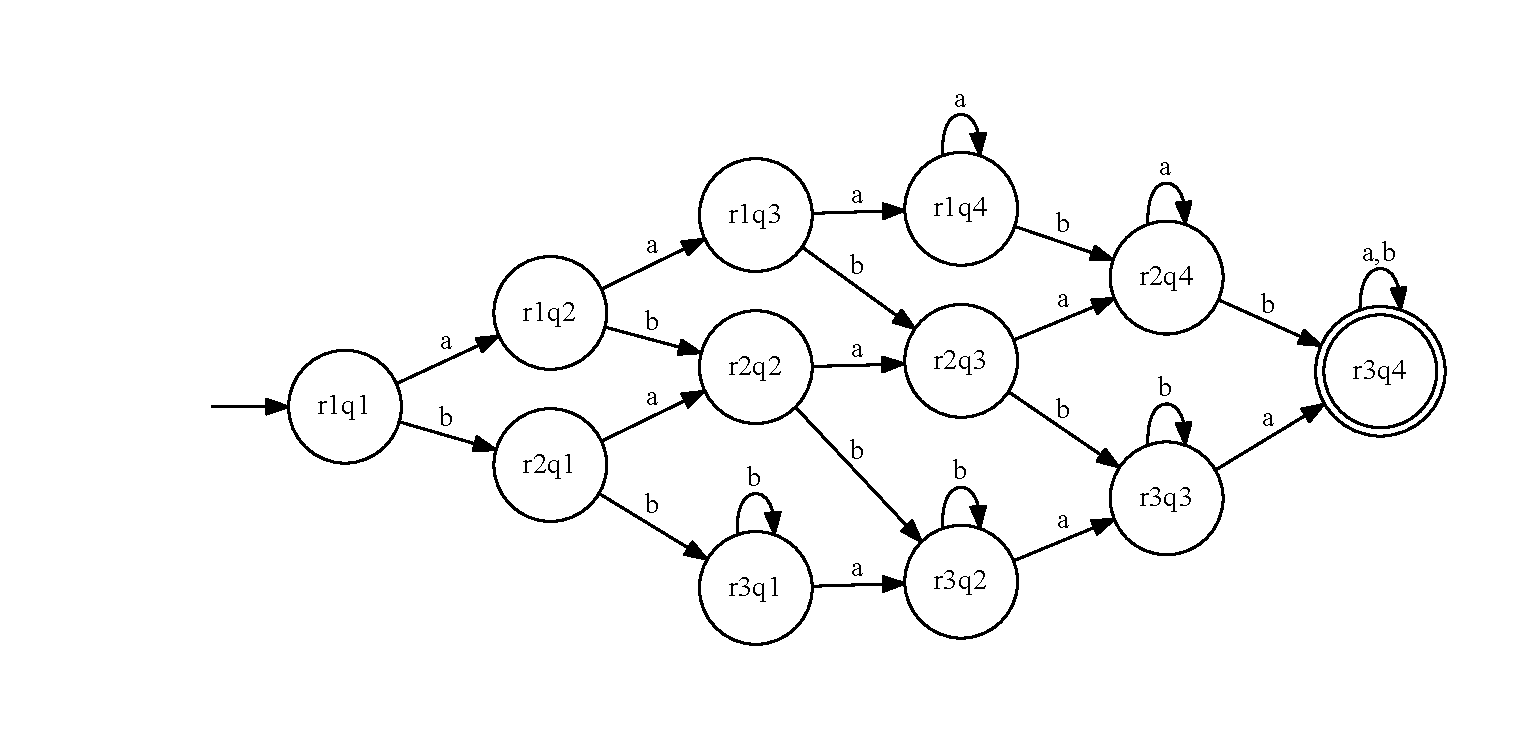
\includegraphics[width=0.9\textwidth]{ac14.pdf}
\caption{State diagram for w has at least three a's and at least two b's.}
\label{3}
\end{figure}
b.Let the state diagram $M_1$ recognize 
$L_1 = \{ w \mid$ w has exactly two a's $\}$:
\begin{figure}[H]
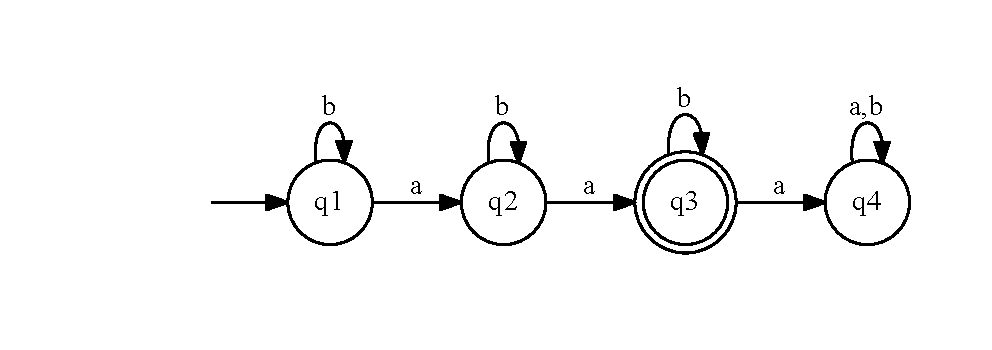
\includegraphics[width=0.9\textwidth]{ba14.pdf}
\caption{State diagram for w has exactly two a's.}
\label{4}
\end{figure} 
Let the state diagram $M_2$ recognize 
$L_2 = \{ w \mid$ w has at least twos b's $\}$:
\begin{figure}[H]
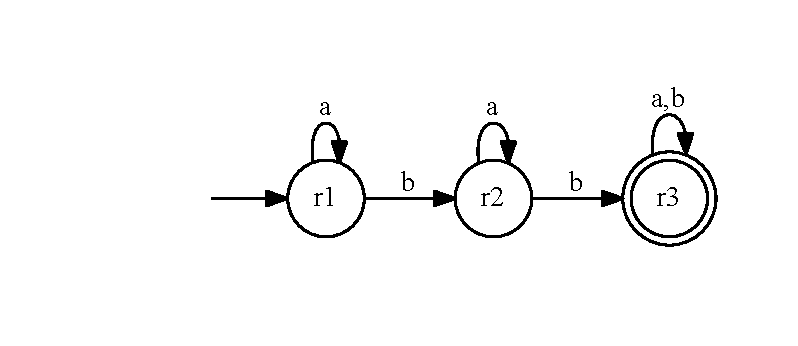
\includegraphics[width=0.9\textwidth]{ab14.pdf}
\caption{State diagram for w has at least two b's.}
\label{5}
\end{figure}
The machine M will accept the input if and only if both $M_1$ and $M_2$ accept. Because language L is the intersection $L_1$ and $L_2$.
The state diagram of M that recognizes the language. $L = \{ w \mid$ w has exactly two a's and at least two b's$\}$: 
\begin{figure}[H]
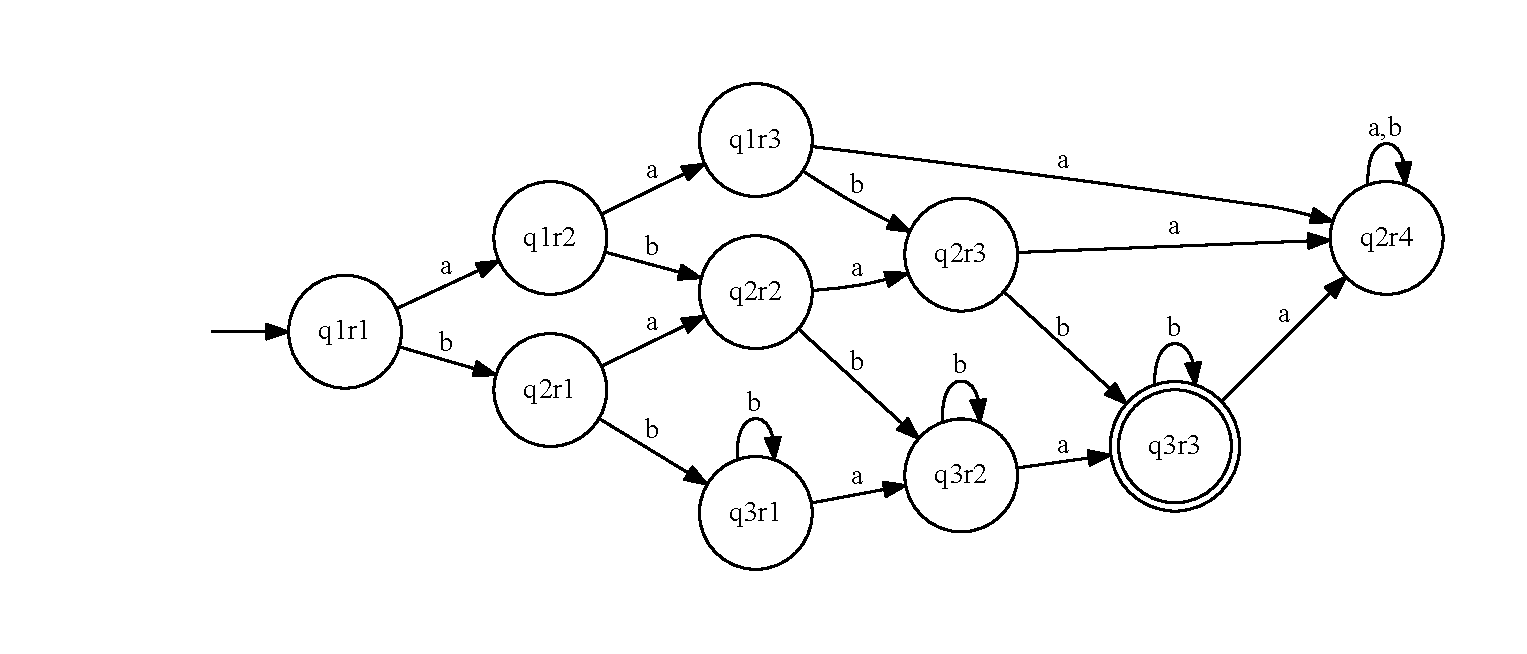
\includegraphics[width=0.9\textwidth]{bb14.pdf}
\caption{State diagram for w exactly two a's and at least two b's.}
\label{6}
\end{figure}
c.Let the state diagram $M_1$ recognize 
$L_1 = \{ w \mid$ w has an even number of a's $\}$:
\begin{figure}[H]
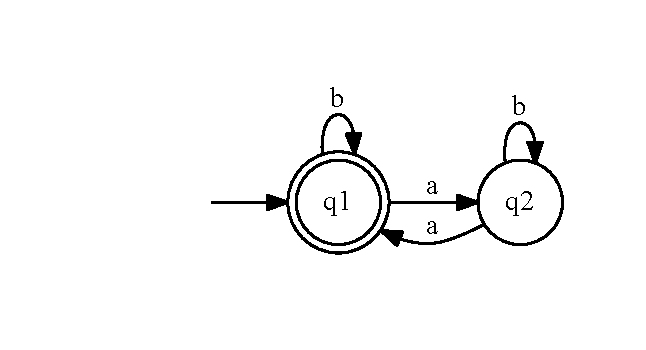
\includegraphics[width=0.9\textwidth]{ca14.pdf}
\caption{State diagram for w has an even number of a's.}
\label{7}
\end{figure} 
Let the state diagram $M_2$ recognize 
$L_2 = \{ w \mid$ w has one or two b's $\}$:
\begin{figure}[H]
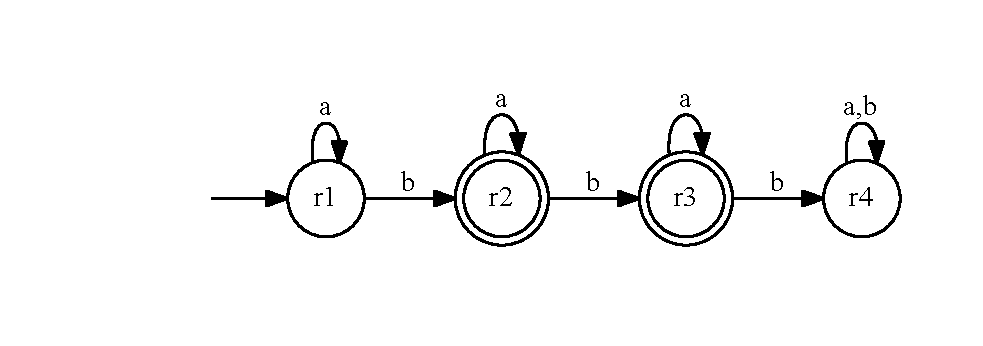
\includegraphics[width=0.9\textwidth]{cb14.pdf}
\caption{State diagram for w has one or two b's.}
\label{8}
\end{figure}
The machine M will accept the input if and only if both $M_1$ and $M_2$ accept. Because language L is the intersection $L_1$ and $L_2$.
The state diagram of M that recognizes the language. $L = \{ w \mid$ w has an even number of a's and one or two b's$\}$: 
\begin{figure}[H]
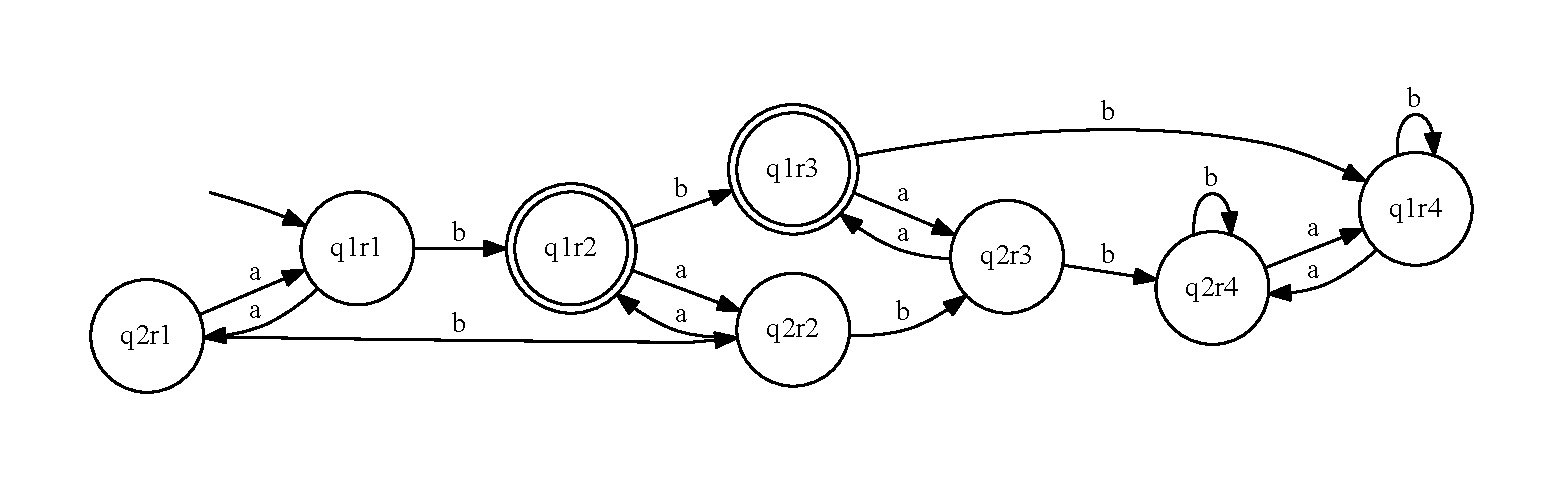
\includegraphics[width=0.9\textwidth]{cc14.pdf}
\caption{State diagram for w has an even number of a's and at least two b's.}
\label{9}
\end{figure}
\item[1.5]
b. This DFA recognizes $L = \{ w \mid$ w contains the substring baba$\}$:
\begin{figure}[H]
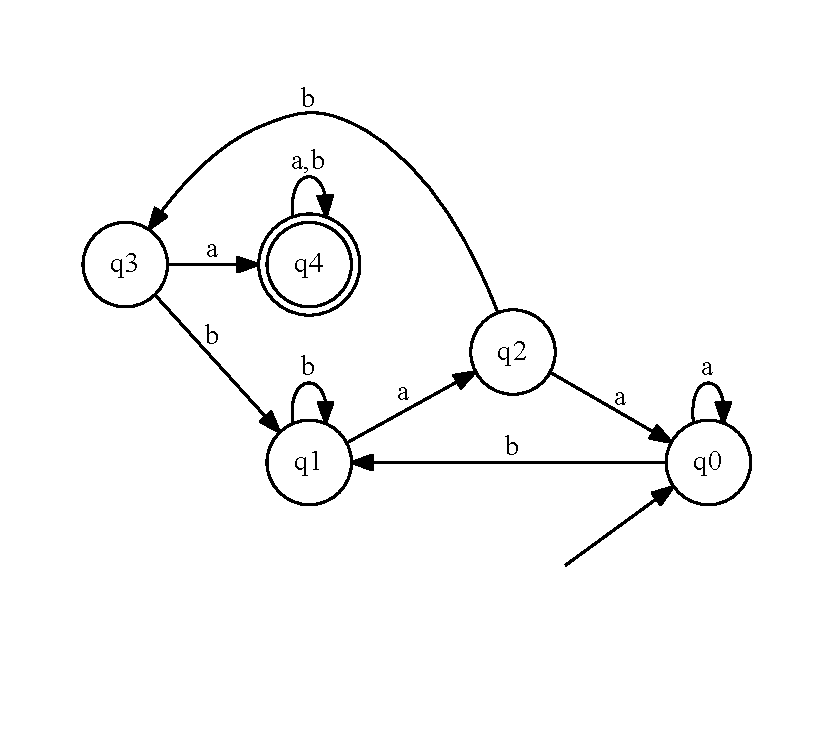
\includegraphics[width=0.9\textwidth]{ba15.pdf}
\caption{State diagram for w contains the substring baba .}
\label{10}
\end{figure}
This DFA recognizes $L = \{ w \mid$ w does not contain the substring baba$\}$:
\begin{figure}[H]
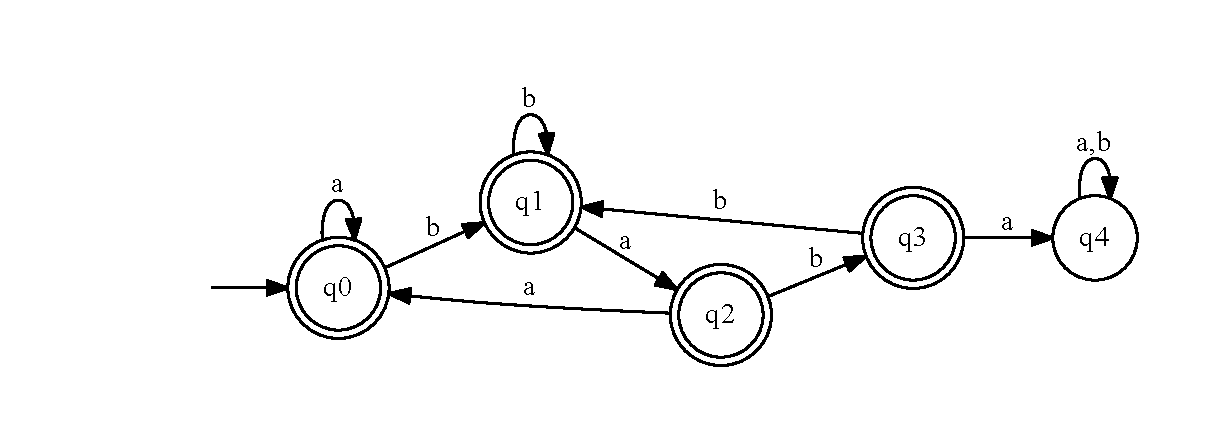
\includegraphics[width=0.9\textwidth]{bb15.pdf}
\caption{State diagram for w does not contain the substring baba .}
\label{11}
\end{figure}
c. This DFA recognizes $L = \{ w \mid$ w contains either the substring ab or ba$\}$:
\begin{figure}[H]
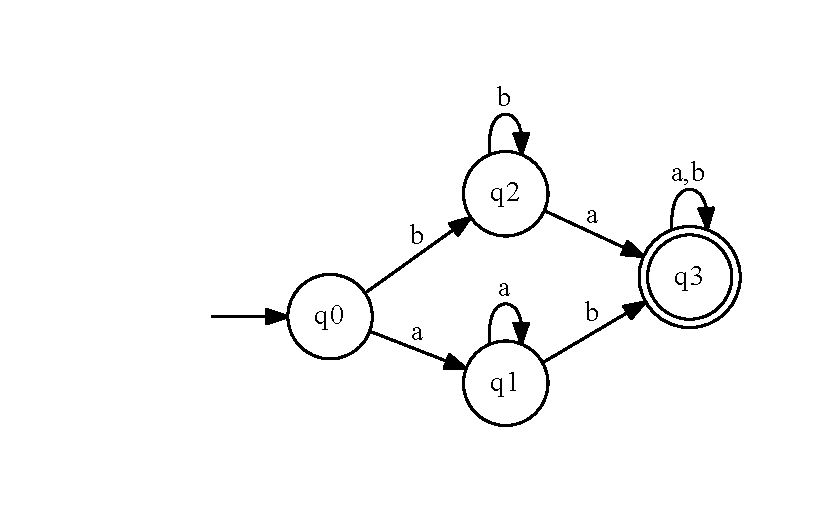
\includegraphics[width=0.9\textwidth]{ca15.pdf}
\caption{State diagram for w contains either the substring ab or ba .}
\label{12}
\end{figure}
This DFA recognizes $L = \{ w \mid$ w contains neither the substring ab nor ba $\}$:
\begin{figure}[H]
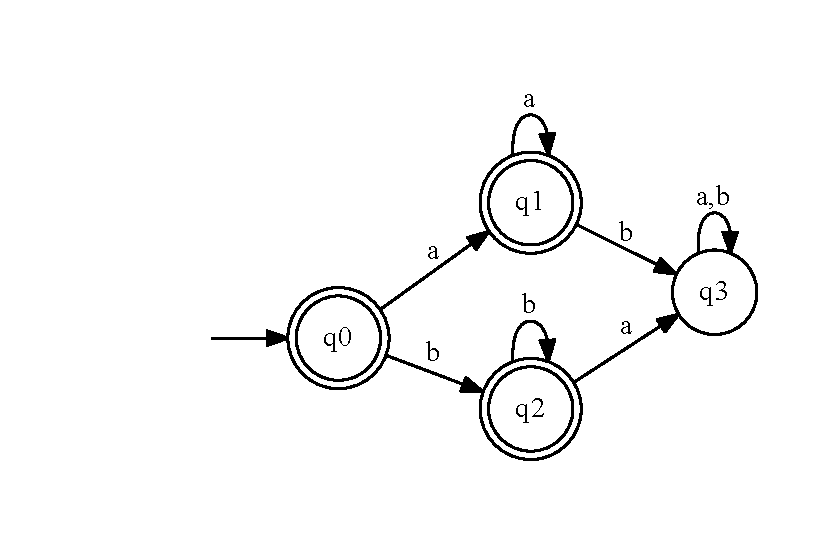
\includegraphics[width=0.9\textwidth]{cb15.pdf}
\caption{State diagram for w contains neither the substring ab nor ba .}
\label{13}
\end{figure}
d. This DFA recognizes $L = \{ w \mid$ w is any string not in $a^* b^*$ $\}$:
\begin{figure}[H]
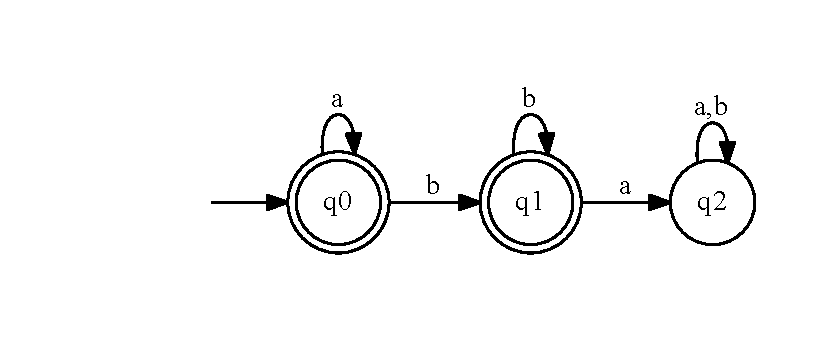
\includegraphics[width=0.9\textwidth]{da15.pdf}
\caption{State diagram for  w is any string not in $a^* b^*$ }
\label{14}
\end{figure}
This DFA recognizes $L = \{ w \mid$ w is any string in $a^* b^*$ $\}$:
\begin{figure}[H]
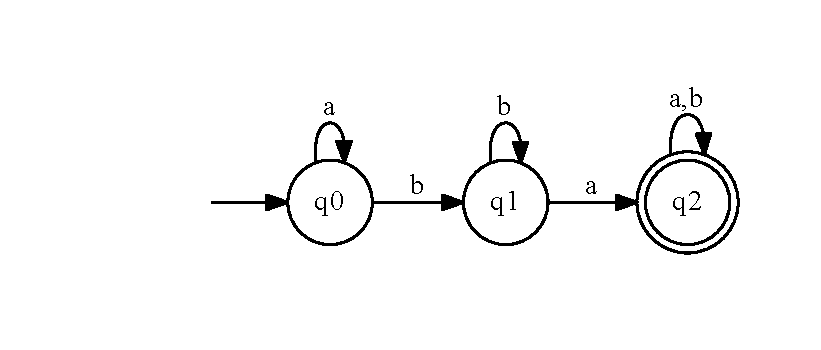
\includegraphics[width=0.9\textwidth]{db15.pdf}
\caption{State diagram for w is any string in $a^* b^*$.}
\label{15}
\end{figure}
\item[1.8]
b.\begin{figure}[H]
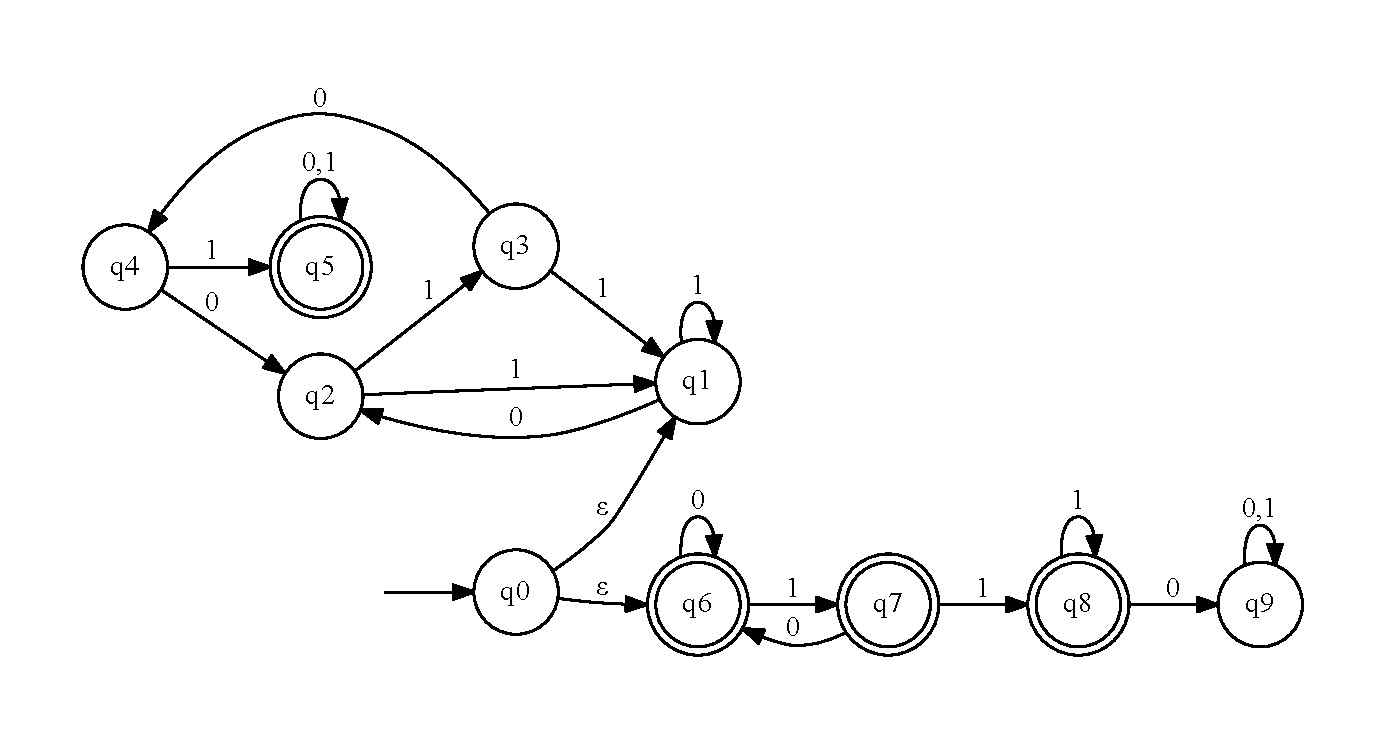
\includegraphics[width=0.9\textwidth]{816.pdf}
\caption{The union of 1.6c and 1.6f.}
\label{16}
\end{figure}
\item[1.9]
a.\begin{figure}[H]
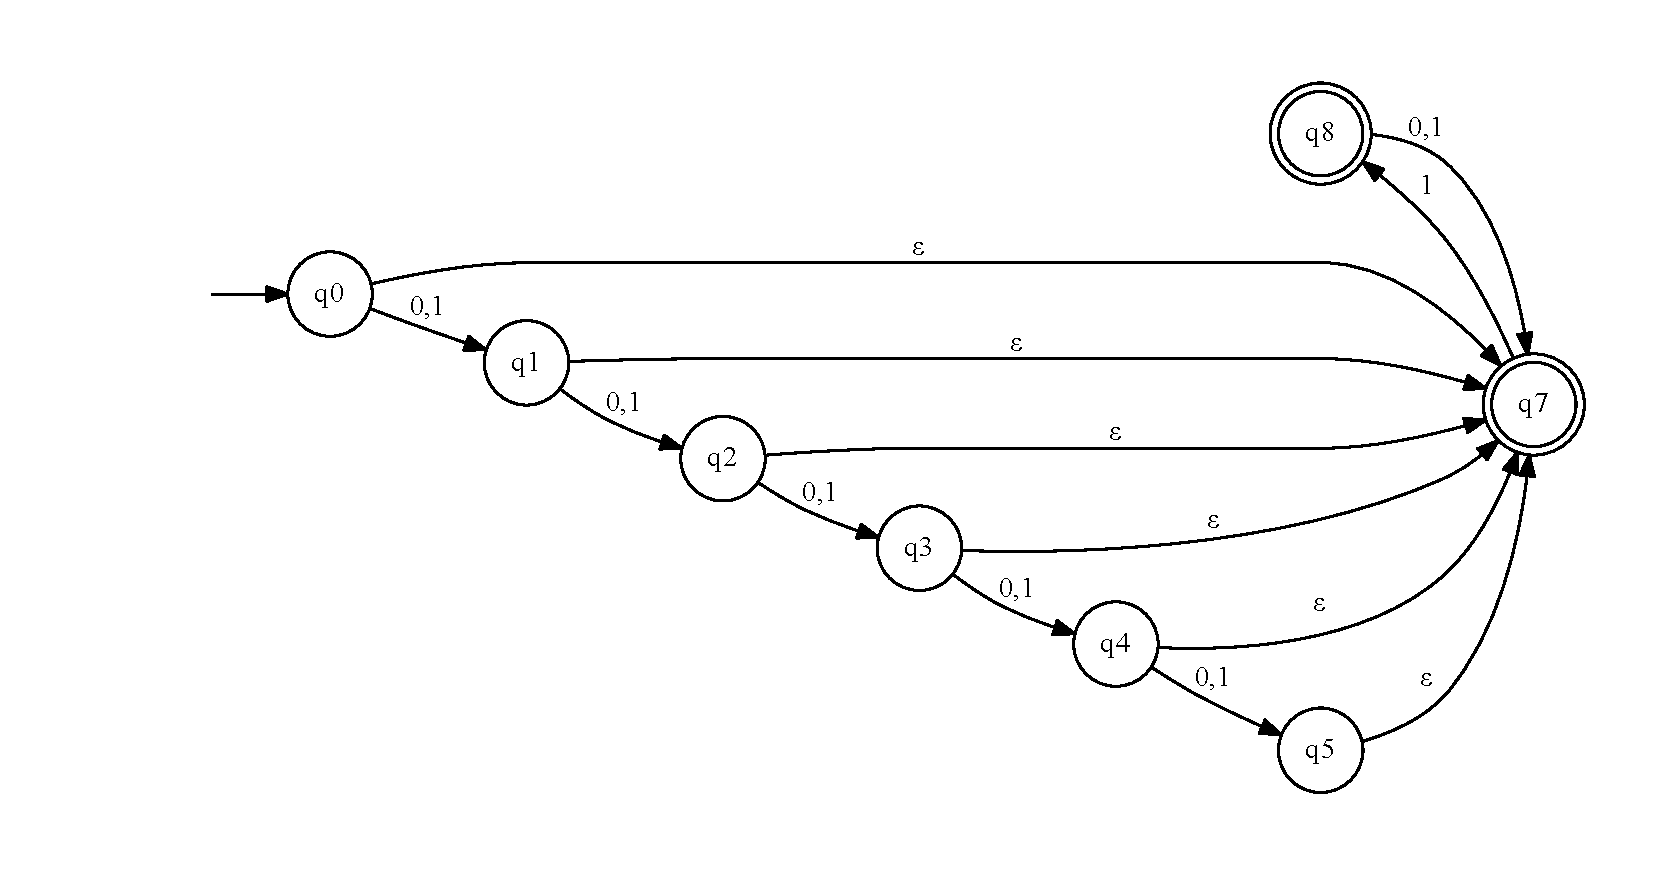
\includegraphics[width=0.9\textwidth]{a19.pdf}
\caption{The concatenation of 1.6g and 1.6i.}
\label{17}
\end{figure}
\item[1.11]\begin{proof}
Let N$=(Q,\Sigma,\delta,q_0,F)$ be any NFA. Create an NFA $N^{'}$ with a single accept state that recognizes the same language as N. $N^{'}$ is exaclty like N except it has $\varepsilon$-transitions from the states corresponding to the accept states of N, to a new accept state $q_{accept}$. State $q_{accept}$ has no emerging transitions.$N^{'}=(Q \cup\{ q_{accept}\}),\Sigma,\delta^{'},q_0,\{ q_{accept}\})$, where for each $q \in Q$ and $a \in \Sigma$.

\[
  \delta^{'}=\begin{cases}
               \delta(q,a)if a \neq \varepsilon or q \not \in F \\\
               \delta(q,a)\cup\{q_{accept}if a = \varepsilon and q \in F \}\\
            \end{cases}
\]
and $\delta^{'}(q_{accept},a)= \emptyset$ for each $a \in \Sigma$
\end{proof}
\item[1.14]
a.Suppose language B  over the alphabet $\Sigma$ has a DFA M$=(Q,\Sigma,\delta,q_1,F)$.Then the a DFA for the complementary language $B^c$ is $M^c=(Q,\Sigma,\delta,q_1,Q-F)$. The reason why M recognizes $M^c$ is as follows. First note that M and $M^c$ have the same transition function $\delta$. Thus, since M is deterministic,$M^c$ is also deterministic. Now consider any string $w \in \Sigma^{*}$.Running M on input string w will result in M ending in some state $r \in Q$. Since M is deterministic there is only one possible state that M can end in on input w. If we run $M^c$ on the same input w, then $M^c$ will end in the same state r since M and $M^c$ have the same transition function. Also since $M^c$ is deterministic there is only one possible ending that $M^c$ can be in on input w.\\
Now suppose that $w \in B$. Then M will accept w, which means that the ending state $r \in F$ ,i.e, r in an accept state of M. But then r$\not \in Q-F$, so $M^{c}$ does not accept w since $M^{c}$ has $Q-F$ as its set of accept states. Similarly suppose that $w \not \in B$. Then M will not accept w, which means that the ending state $r \not \in F$. But then $r \in Q-F$, so $M^{c}$ accepts w. Therefore $M^{c}$ accepts string w if and only if M does not accept string w, so $M^{c}$ recognizes language $M^{c}$. Hence the class of regular languages is closed under complement.\\
b.The NFA M below recognizes the language C$=\{ w \in \Sigma^{*} \mid$ w ends with 00 $\}$, where $\Sigma=\{0,1 \}$. 
\begin{figure}[H]
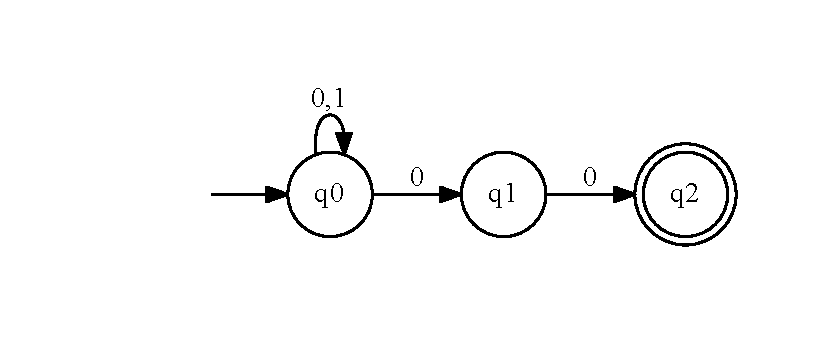
\includegraphics[width=0.9\textwidth]{a114.pdf}
\label{18}
\end{figure}
Swapping the accept and non-accept states of M makes the following NFA $M^{'}$.
\begin{figure}[H]
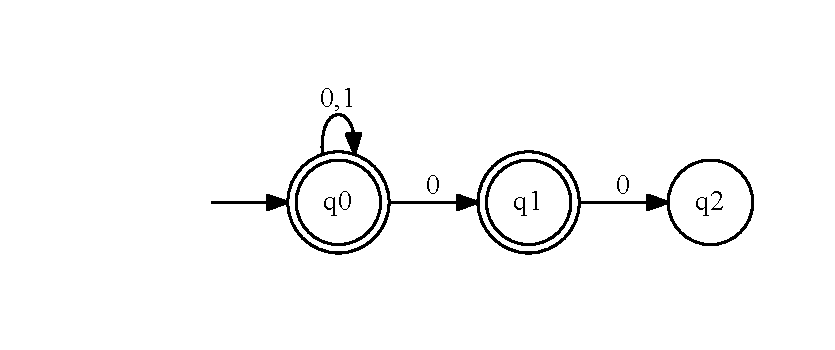
\includegraphics[width=0.9\textwidth]{b114.pdf}
\label{19}
\end{figure}
Note that $M^{'}$ accepts the string,100$\not \in \bar{C} = \{w \mid$ does not end with$ 00 \}$ so $M^{'}$ does not recognize the language $\bar{C}$.\\
The class of languages recognized by NFAs is closed under complement, which we can as follows. Suppose that C is a  recognized by NFA M, i.e., C$=L(M)$. Since every NFA has an equivalent DFA(Theorem 1.19), there is a DFA D such that $L(D)=L(M)=C$. Since every DFA is also an NFA, this then shows that there is an NFA, in particular $\bar{D}$, that recognizes the language $\bar{C}=\bar{L}=\bar{(D)}$. Thus, the class of languages recognized by the  NFA is closed under complement.
\item[1.16]
a.NFA:N$=(Q,\Sigma,\delta,q_0,F)$\\
DFA:M$=(Q^{'},\Sigma^{'},\delta,q^{'}_{0},F^{'})$\\
1.$Q^{'}=P(Q)$\\
$Q^{'}=\{\emptyset,\{1 \},\{2\}, \{1,2 \} \}$\\
$\Sigma^{'}=\Sigma$\\
$\delta^{'}(\emptyset,a)=\emptyset$\\
$\delta^{'}(\emptyset,b)=\emptyset$\\
$\delta^{'}(\{1 \},a)=\delta(1,a)=\{ 1,2\}$\\
$\delta^{'}(\{1 \},b)=\delta(1,b)=\{2\}$\\
$\delta^{'}(\{2 \},a)=\delta(2,a)=\emptyset$\\
$\delta^{'}(\{2 \},b)=\delta(2,b)=\{ 1\}$\\
$\delta^{'}(\{1,2 \},a)=\delta(1,a)\cup \delta(2,a)=\{ 1,2\} \cup \emptyset= \{1,2 \}$\\
$\delta^{'}(\{1,2 \},b)=\delta(1,b)\cup \delta(2,b)=\{2\} \cup 
\{ 1\}= \{1,2 \}$\\
$q^{'}=\{ q_0\}$\\
$q_0= \{ 1\}$\\
$F^{'}=\{R \in Q^{'} \mid R $contains an accept state of N $\}$\\
$F^{'}=\{\{ 1\}, \{1,2 \} \}$
\begin{figure}[H]
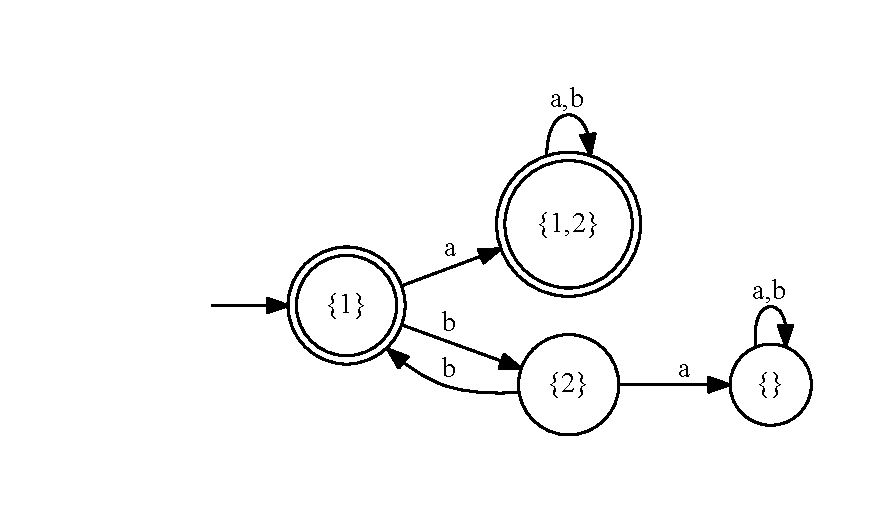
\includegraphics[width=0.9\textwidth]{a116.pdf}
\label{20}
\end{figure}
b.NFA:N$=(Q,\Sigma,\delta,q_0,F)$\\
DFA:M$=(Q^{'},\Sigma^{'},\delta,q^{'}_{0},F^{'})$\\
1.$Q^{'}=P(Q)$\\
$Q^{'}=\{\emptyset,\{1 \},\{2\},\{3 \} \{1,2 \},\{ 1,3\}, \{2,3 \},\{1,2,3 \} \}$\\
$\Sigma^{'}=\Sigma$\\
$\delta^{'}(\emptyset,a)=\emptyset$\\
$\delta^{'}(\emptyset,b)=\emptyset$\\
$\delta^{'}(\{1,2 \},a)=\delta(\{1\},a)\cup \delta(\{2\},a)= \{1,2,3 \}$\\
$\delta^{'}(\{1,2 \},b)=\delta(\{1\},a)\cup \delta(\{2\},b)= \emptyset$\\
$\delta^{'}(\{2,3 \},a)=\delta(\{2\},a)\cup \delta(\{3\},a)=\{1,2\}$\\
$\delta^{'}(\{2,3 \},b)=\delta(\{2\},b)\cup \delta(\{3\},b)=\{2,3\}$\\
$\delta^{'}(\{1,2,3 \},a)=\delta(\{1\},a)\cup \delta(\{2\},a)\cup	(\{ 3\},a)=\{1,2,3\}$\\
$\delta^{'}(\{1,2,3 \},b)=\delta(\{1\},b)\cup \delta(\{2\},b)\cup	(\{ 3\},b)=\{2,3\}$\\
$q^{'}=\{ q_0\}$\\
$q_0= \{ 1,2\}$\\
$F^{'}=\{R \in Q^{'} \mid R $contains an accept state of N $\}$\\
$F^{'}=\{\{ 1,2\}, \{2,3 \}, \{1,2,3 \} \}$
\begin{figure}[H]
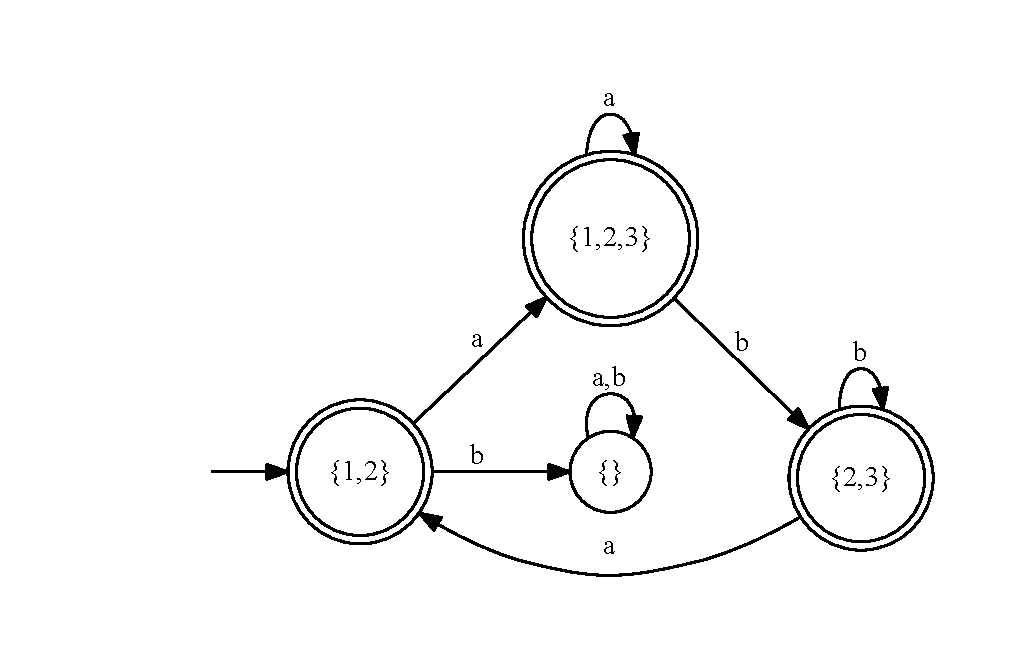
\includegraphics[width=0.9\textwidth]{b116.pdf}
\label{21}
\end{figure}
\item[1.18]
Let $\Sigma= ( 0\cup 1)$ and $\Sigma^*=(0 \cup 1)^*$\\
a.$1\Sigma^*0$\\
b.$\Sigma^* 1 \Sigma^*  1 \Sigma^* 1 \Sigma^* $\\
c.$\Sigma^* 0101 \Sigma^* $\\
d.$\Sigma  \Sigma  0 \Sigma^*  $\\
e.$(0 \cup 1 \Sigma)(\Sigma\Sigma)^*$\\
f.$0^*(10^{+})^*1^*$\\
g.$(\varepsilon \cup \Sigma)^{5}$\\
h.$\varepsilon \cup	\Sigma \cup 0 \Sigma \cup 10 \cup 0 \Sigma \Sigma \cup 10 \Sigma \cup 110 \cup \Sigma^{3} \Sigma^{+}$\\
i.$(1 \Sigma)^* (\varepsilon \cup 1 )$\\
j.$00^{+} \cup 100^{+} \cup 0^{+}10^{+} \cup 00^{+}1$\\
k.$0 \cup \varepsilon$\\
l.$1^{*}(01^{*}01^{*}) \cup 0^{*}10^{*}10^{*}$\\
m.$\emptyset$\\
n.$\Sigma^{+}$
\item[1.21]
a.$a^*b(a \cup ba^*b)^*$
\begin{figure}[H]
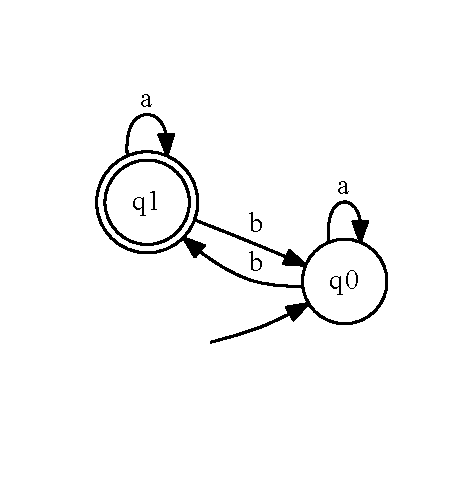
\includegraphics[width=0.5\textwidth]{aa21.pdf}
\caption{The starting finite automata.}
\label{22}
\end{figure}
\begin{figure}[H]
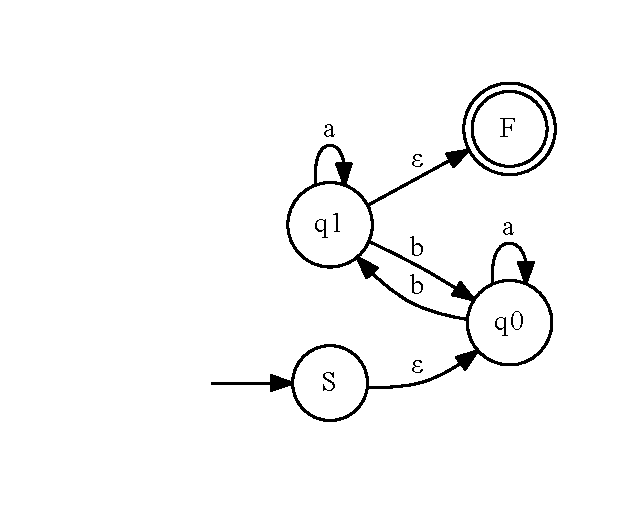
\includegraphics[width=0.5\textwidth]{ab21.pdf}
\caption{The adding a new start and accept states.}
\label{23}
\end{figure}
\begin{figure}[H]
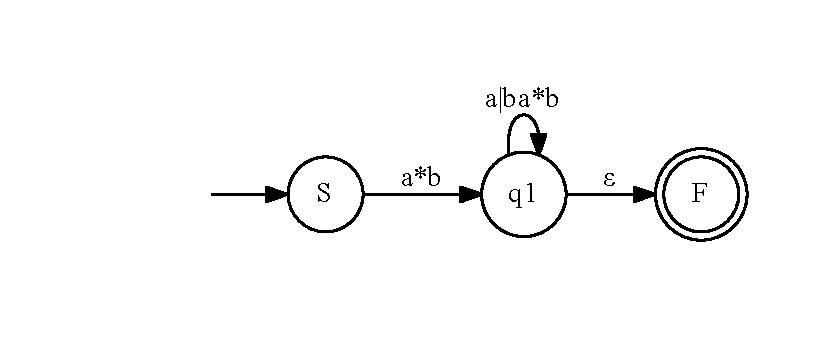
\includegraphics[width=0.5\textwidth]{ac21.pdf}
\caption{After removing q0.}
\label{24}
\end{figure}
\begin{figure}[H]
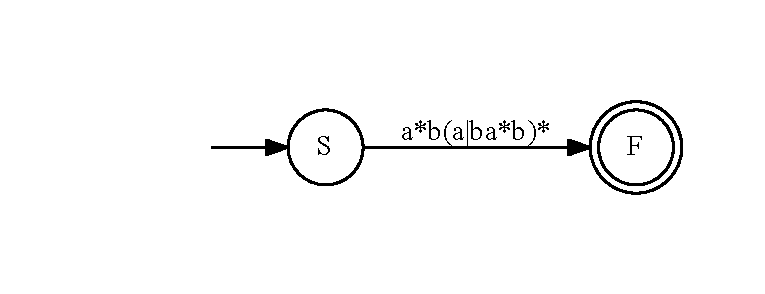
\includegraphics[width=0.5\textwidth]{ad21.pdf}
\caption{After removing q1.}
\label{25}
\end{figure}
b.$\varepsilon \cup(a \cup b)a^* b ((a(a \cup b) \cup b)a^* b )^* (\varepsilon \cup a)$
\begin{figure}[H]
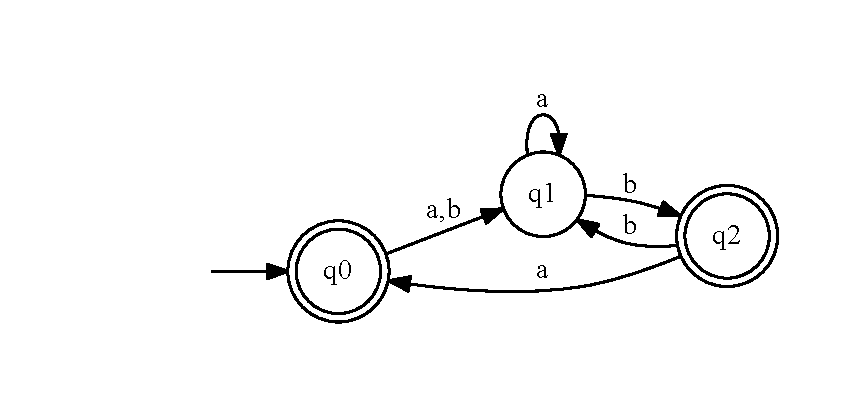
\includegraphics[width=0.5\textwidth]{bba21.pdf}
\caption{The starting finite automata.}
\label{26}
\end{figure}
\begin{figure}[H]
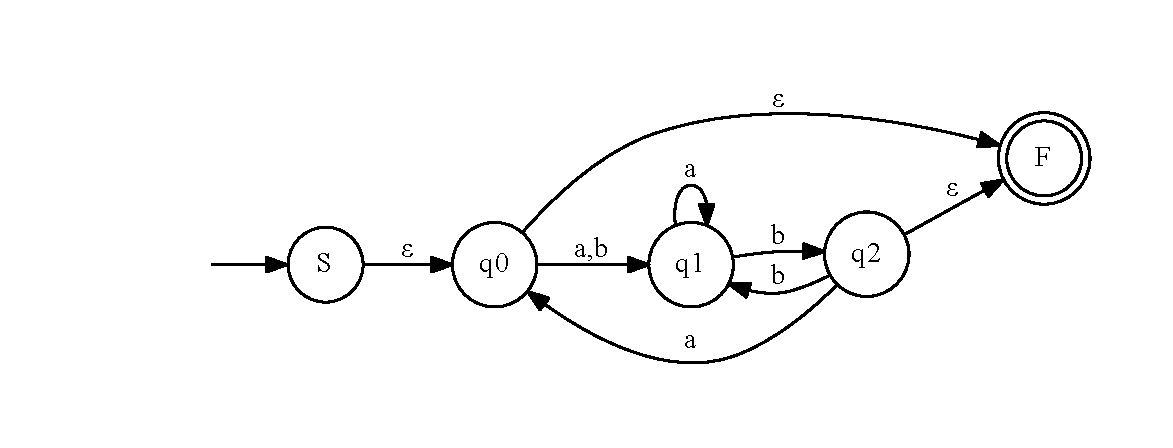
\includegraphics[width=0.8\textwidth]{bbb21.pdf}
\caption{After adding a new start and end state.}
\label{27}
\end{figure}
\begin{figure}[H]
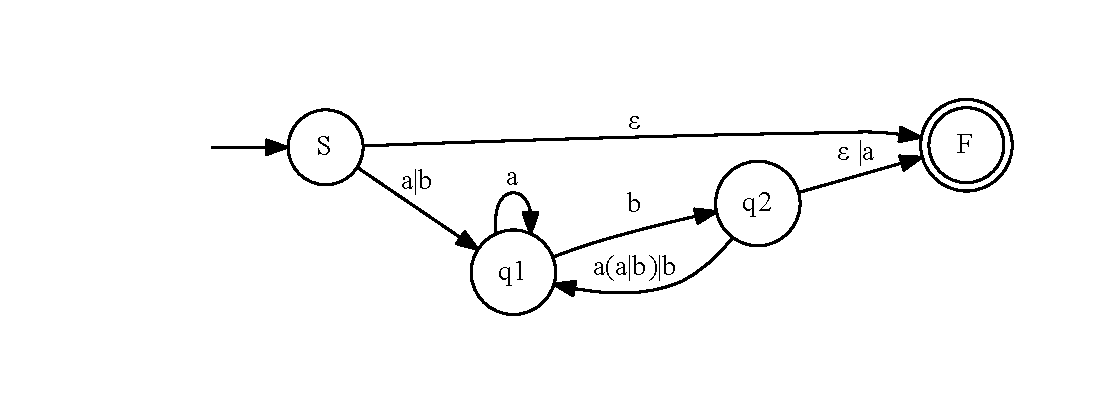
\includegraphics[width=0.8\textwidth]{bbc21.pdf}
\caption{After removing q0.}
\label{28}
\end{figure}
\begin{figure}[H]
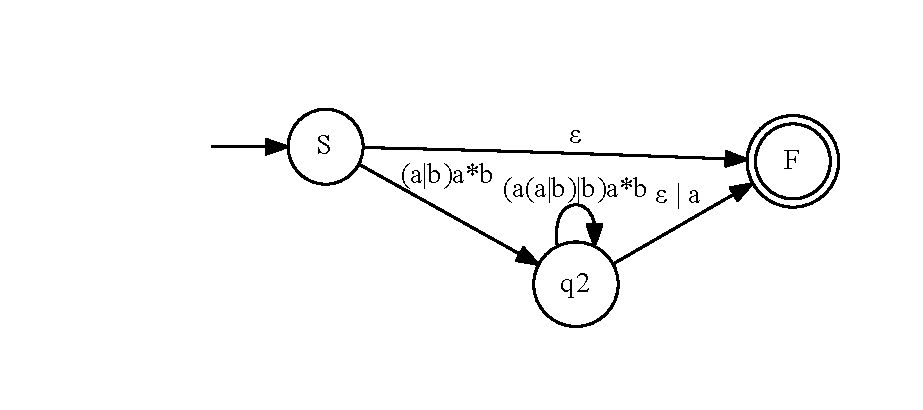
\includegraphics[width=0.8\textwidth]{bbd21.pdf}
\caption{After removing q1.}
\label{29}
\end{figure}
\begin{figure}[H]
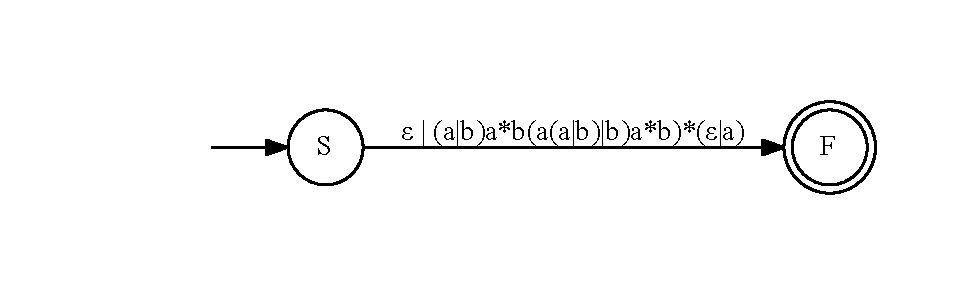
\includegraphics[width=0.8\textwidth]{bbe21.pdf}
\caption{After removing q2.}
\label{30}
\end{figure}
\item[1.28]
a.\begin{figure}[H]
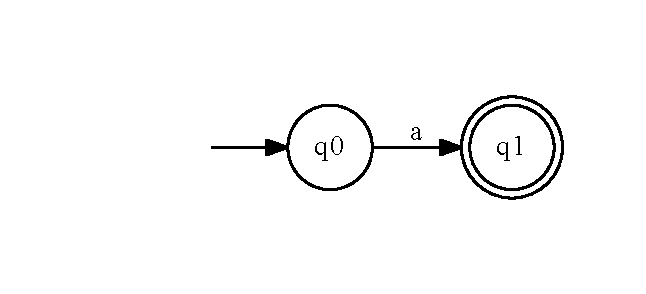
\includegraphics[width=0.8\textwidth]{aa28.pdf}
\caption{The NFA for a.}
\label{31}
\end{figure}
\begin{figure}[H]
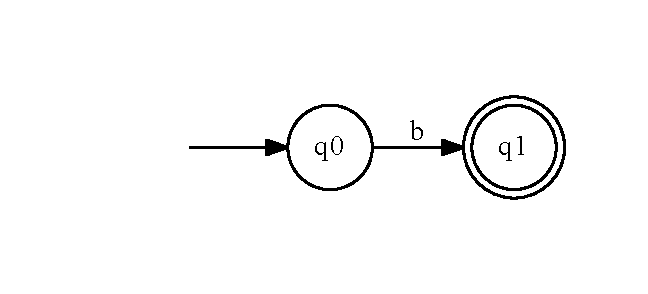
\includegraphics[width=0.8\textwidth]{ab28.pdf}
\caption{The NFA for b.}
\label{32}
\end{figure}
\begin{figure}[H]
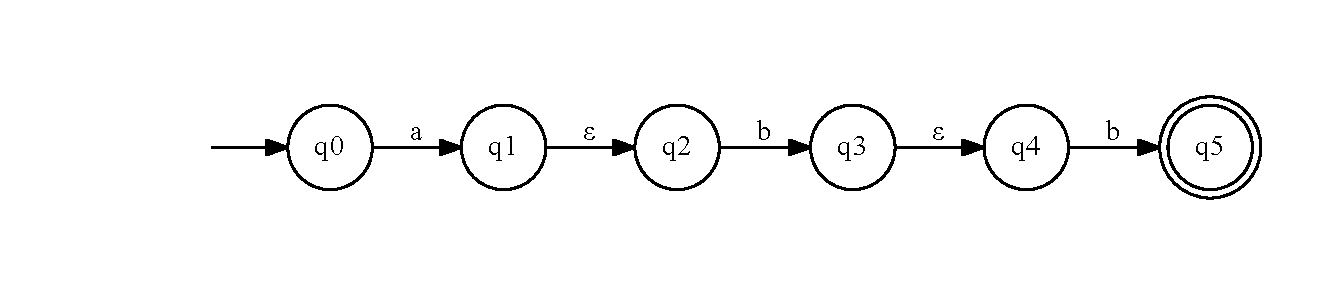
\includegraphics[width=0.8\textwidth]{ac28.pdf}
\caption{The NFA for abb.}
\label{33}
\end{figure}
\begin{figure}[H]
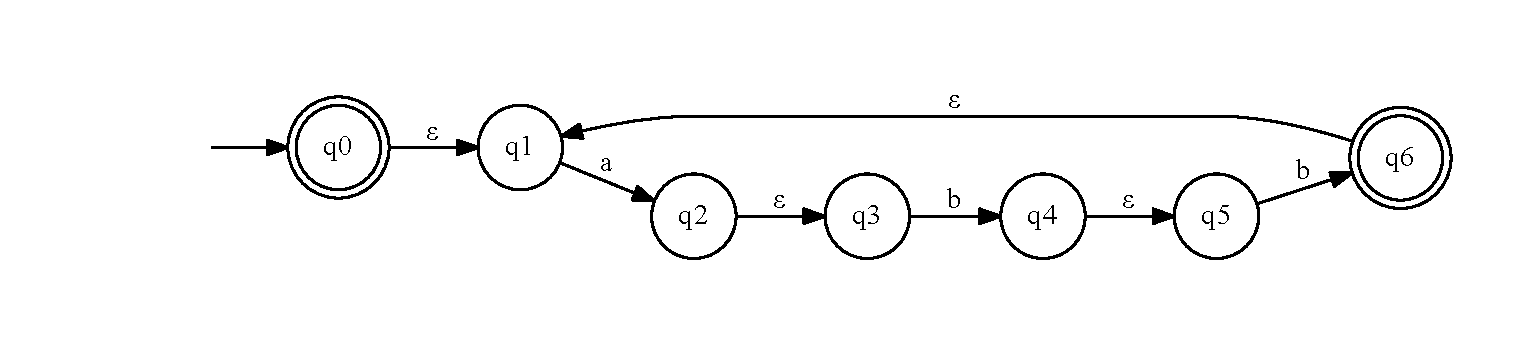
\includegraphics[width=0.8\textwidth]{ad28.pdf}
\caption{The NFA for (abb)*.}
\label{34}
\end{figure}
\begin{figure}[H]
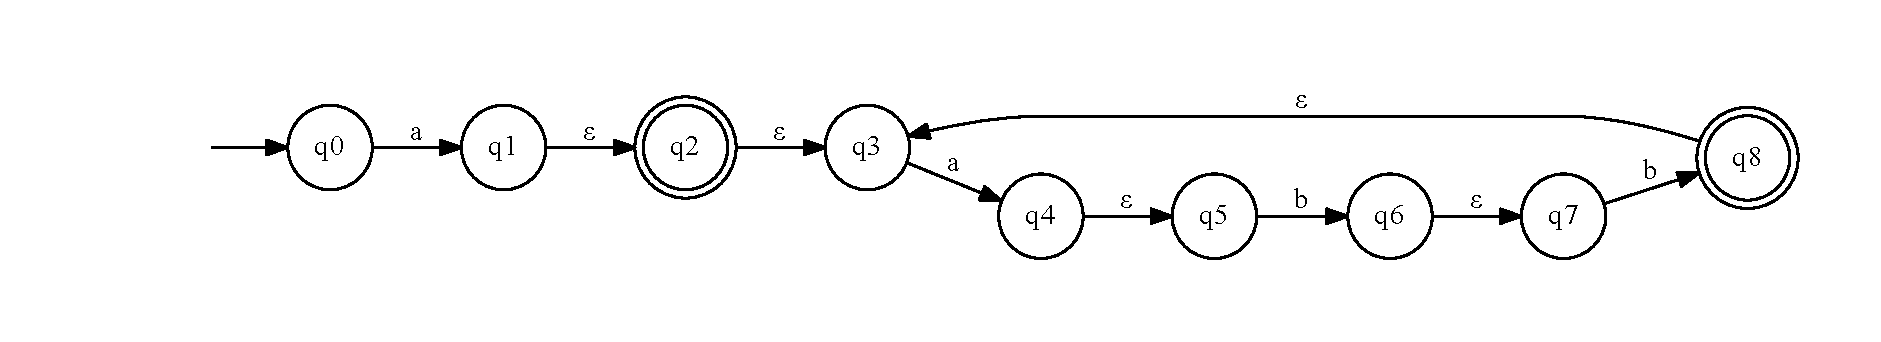
\includegraphics[width=0.8\textwidth]{ae28.pdf}
\caption{The NFA for a(abb)*.}
\label{35}
\end{figure}
\begin{figure}[H]
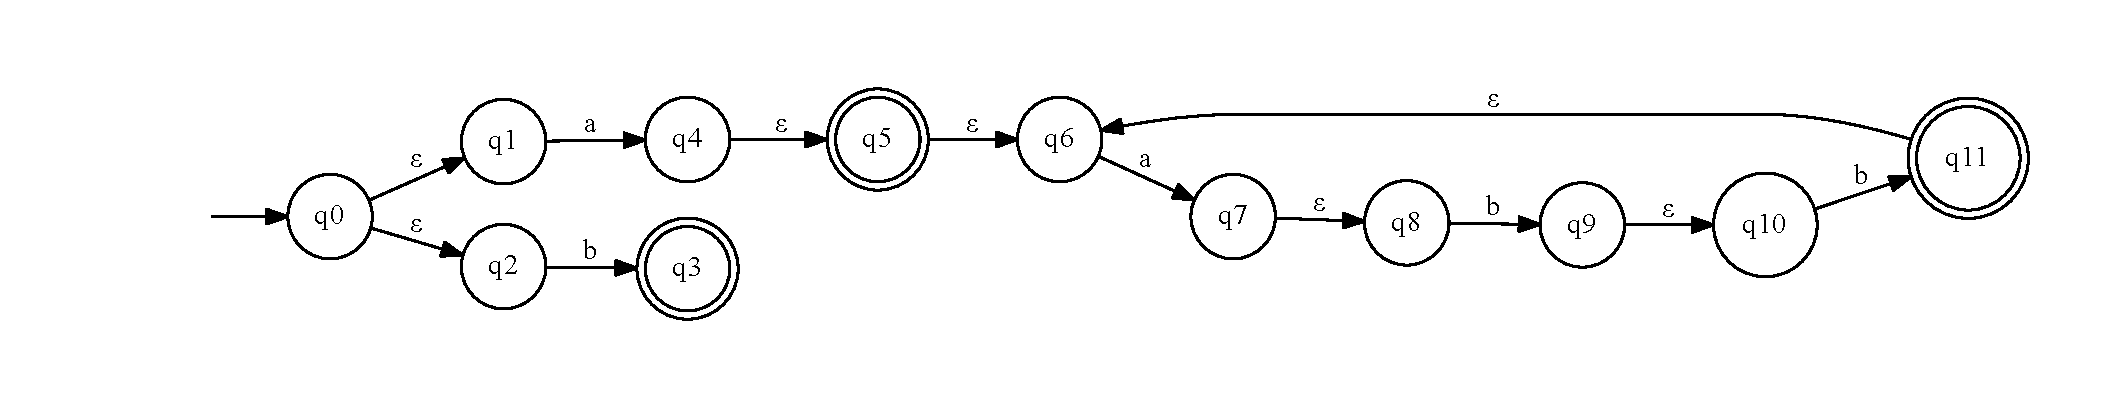
\includegraphics[width=0.8\textwidth]{af28.pdf}
\caption{The NFA for a(abb*)$\cup$b.}
\label{36}
\end{figure}
b.\begin{figure}[H]
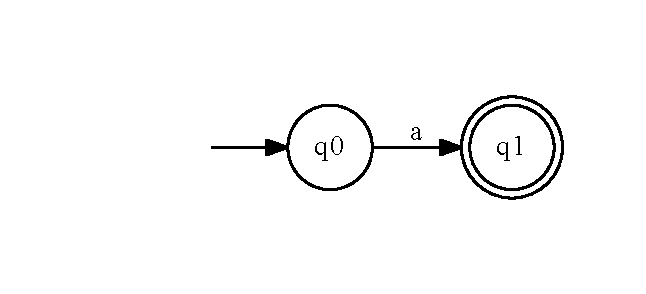
\includegraphics[width=0.8\textwidth]{aa28.pdf}
\caption{The NFA for a.}
\label{37}
\end{figure}
\begin{figure}[H]
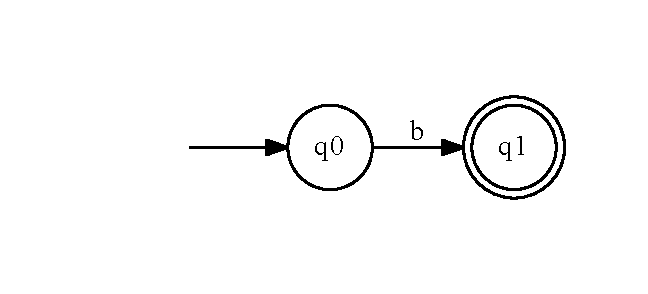
\includegraphics[width=0.8\textwidth]{ab28.pdf}
\caption{The NFA for b.}
\label{38}
\end{figure}
\begin{figure}[H]
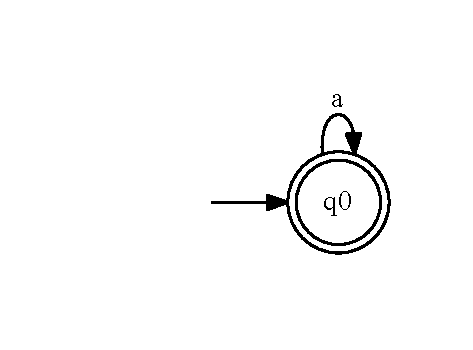
\includegraphics[width=0.7\textwidth]{bc28.pdf}
\caption{The NFA for a*.}
\label{39}
\end{figure}
\begin{figure}[H]
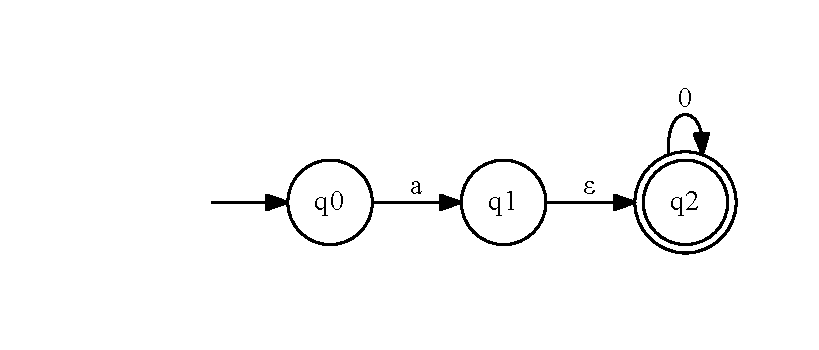
\includegraphics[width=0.8\textwidth]{bd28.pdf}
\caption{The NFA for $a^{+}$.}
\label{40}
\end{figure}
\begin{figure}[H]
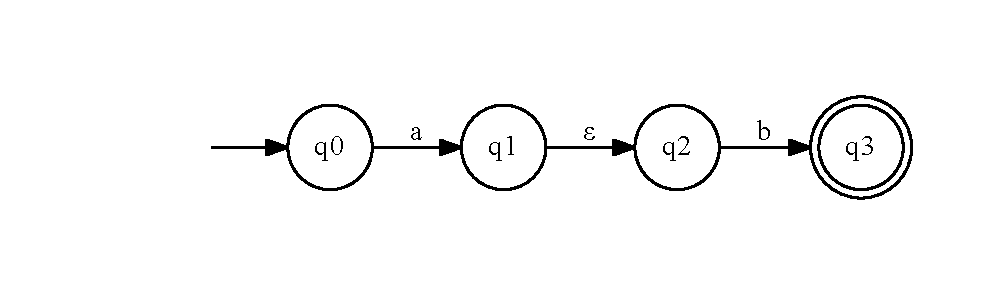
\includegraphics[width=0.8\textwidth]{be28.pdf}
\caption{The NFA for ab.}
\label{41}
\end{figure}
\begin{figure}[H]
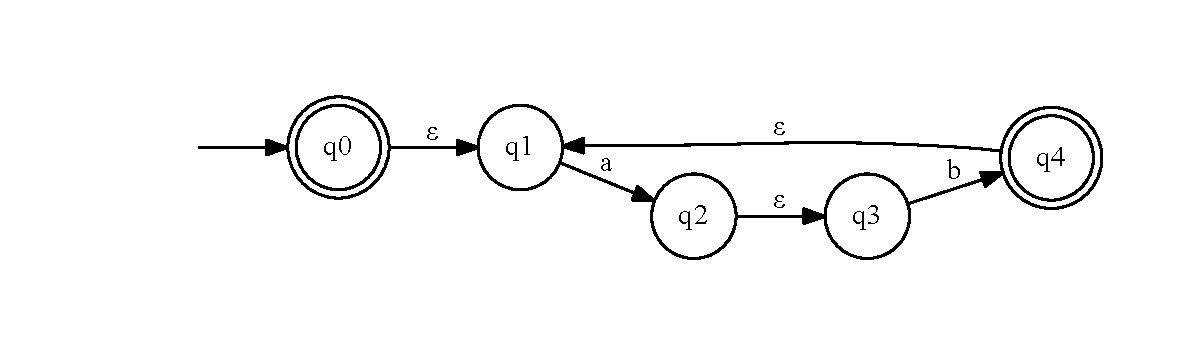
\includegraphics[width=0.8\textwidth]{bf28.pdf}
\caption{The NFA for (ab)*.}
\label{42}
\end{figure}
\begin{figure}[H]
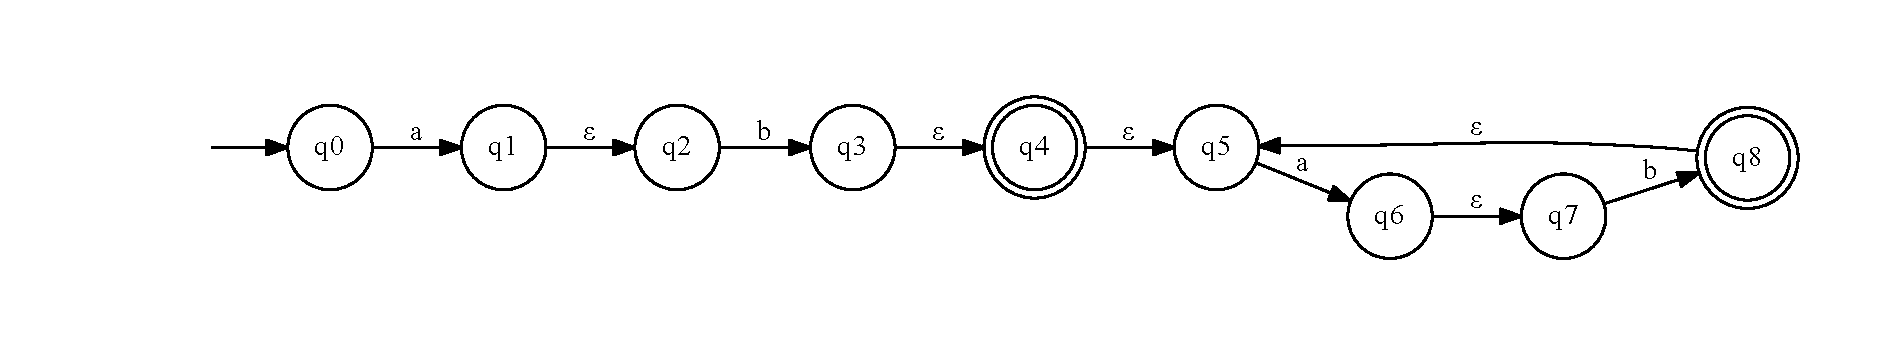
\includegraphics[width=0.8\textwidth]{bg28.pdf}
\caption{The NFA for $(ab)^{+}$.}
\label{43}
\end{figure}
\begin{figure}[H]
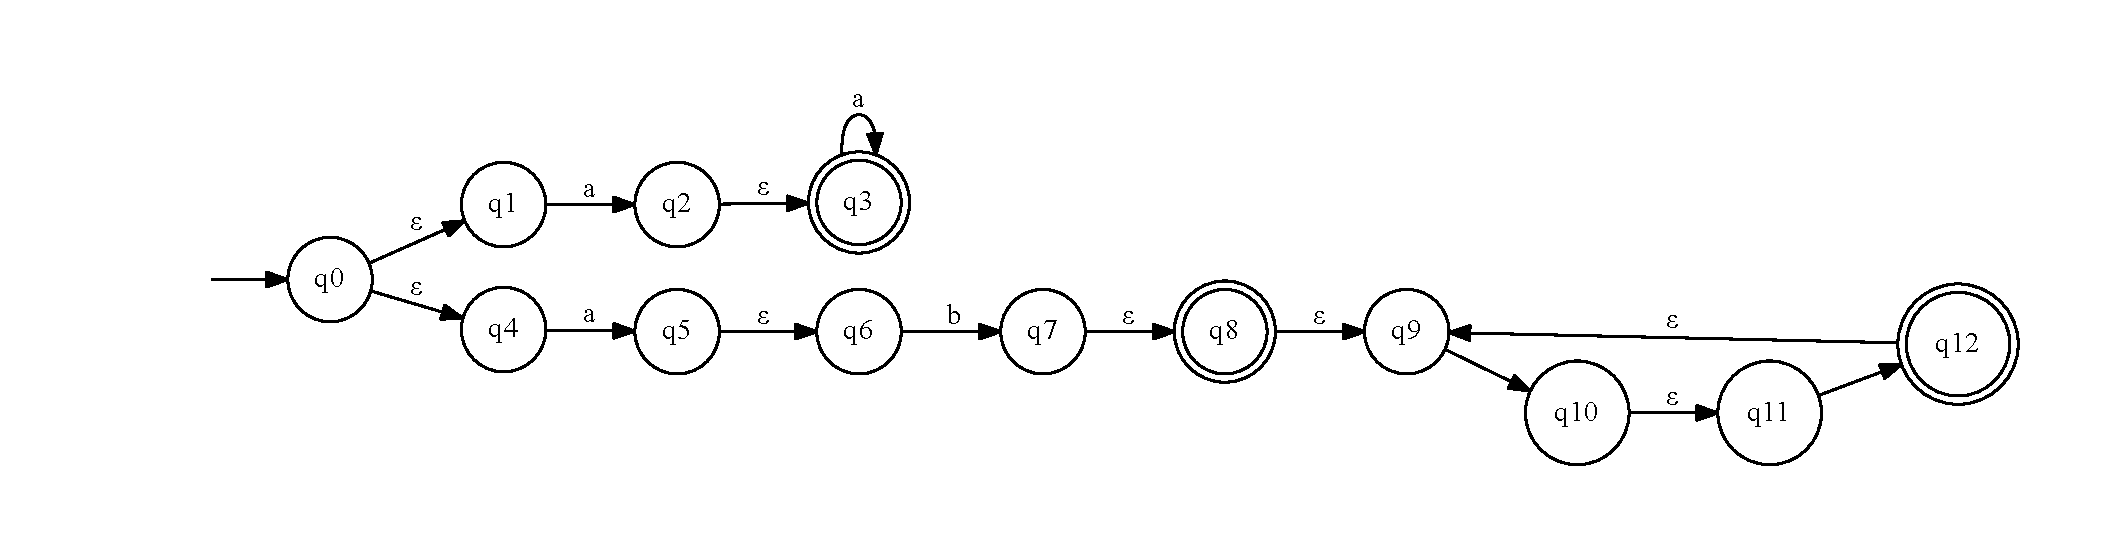
\includegraphics[width=0.8\textwidth]{bh28.pdf}
\caption{The NFA for $a^{+} \cup (ab)^{+}$.}
\label{44}
\end{figure}
c.\begin{figure}[H]
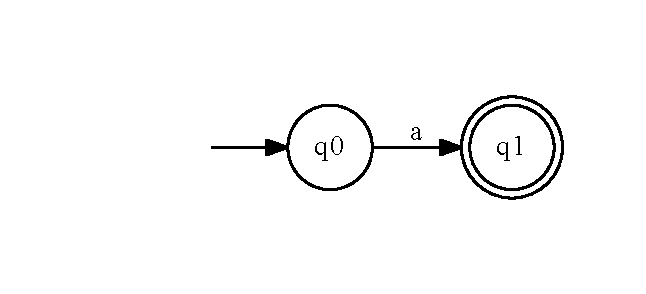
\includegraphics[width=0.8\textwidth]{aa28.pdf}
\caption{The NFA for a.}
\label{45}
\end{figure}
\begin{figure}[H]
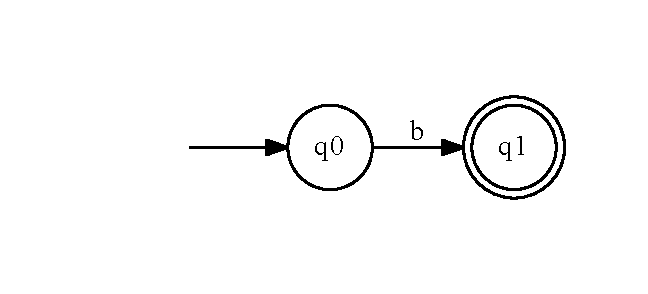
\includegraphics[width=0.8\textwidth]{ab28.pdf}
\caption{The NFA for b.}
\label{46}
\end{figure}
\begin{figure}[H]
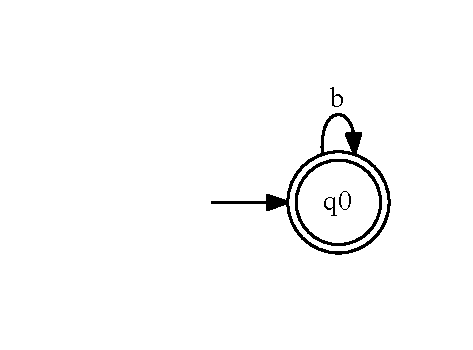
\includegraphics[width=0.7\textwidth]{ca28.pdf}
\caption{The NFA for b*.}
\label{47}
\end{figure}
\begin{figure}[H]
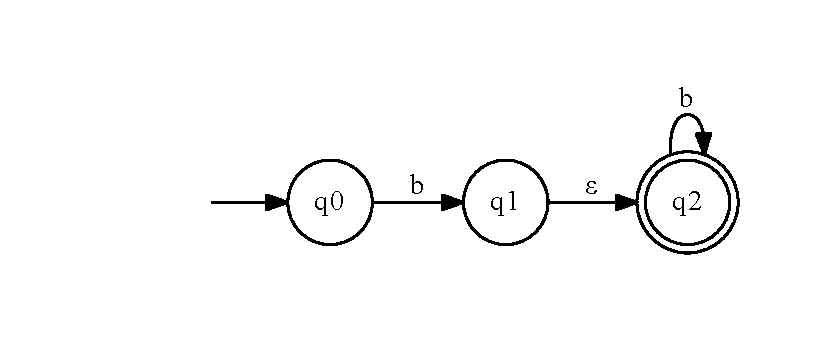
\includegraphics[width=0.7\textwidth]{cb28.pdf}
\caption{The NFA for $b^{+}$.}
\label{48}
\end{figure}
\begin{figure}[H]
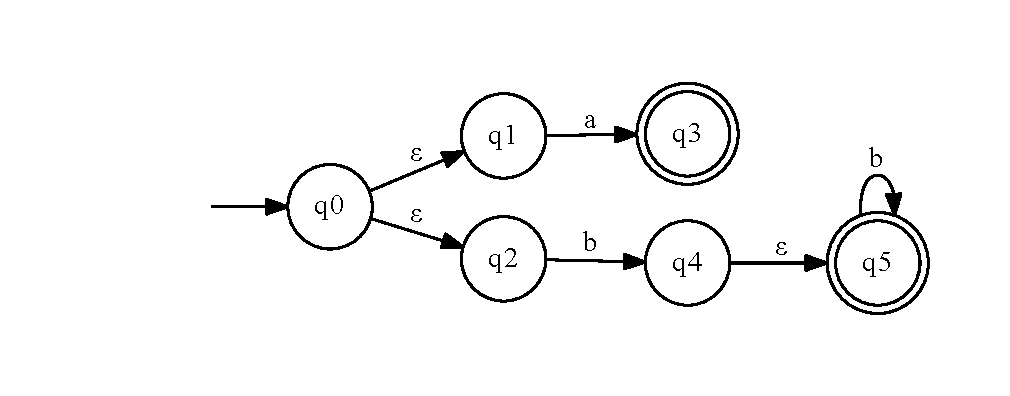
\includegraphics[width=0.7\textwidth]{cc28.pdf}
\caption{The NFA for $a \cup b^{+}$.}
\label{49}
\end{figure}
\begin{figure}[H]
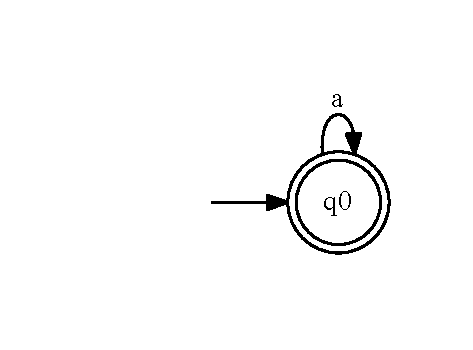
\includegraphics[width=0.7\textwidth]{bc28.pdf}
\caption{The NFA for a*.}
\label{50}
\end{figure}
\begin{figure}[H]
\includegraphics[width=0.7\textwidth]{cd28.pdf}
\caption{The NFA for $a^{+}$.}
\label{51}
\end{figure}
\begin{figure}[H]
\includegraphics[width=0.7\textwidth]{ce28.pdf}
\caption{The NFA for $a^{+}b^{+}$.}
\label{52}
\end{figure}
\begin{figure}[H]
\includegraphics[width=0.9\textwidth]{cf28.pdf}
\caption{The NFA for $(a \cup b^{+})a^{+}b^{+}$.}
\label{53}
\end{figure}
\end{enumerate}
\end{document}
